%% main.tex — Unified FPGA Quantum Simulator Paper
%% Document class: sn-jnl (Springer Nature journal template)
%% Compile: pdflatex main && bibtex main && pdflatex main && pdflatex main

\documentclass[pdflatex,sn-mathphys-num]{sn-jnl}

%% ---- packages ---------------------------------------------------------------
\usepackage{amsmath,amssymb,bm}
\usepackage{graphicx}
\usepackage{booktabs}
\usepackage{multirow}
\usepackage{algorithm}
\usepackage{algpseudocode}
\usepackage{hyperref}
\usepackage{siunitx}

%% ---- macros -----------------------------------------------------------------
\newcommand{\ket}[1]{|#1\rangle}
\newcommand{\bra}[1]{\langle#1|}
\newcommand{\braket}[2]{\langle#1|#2\rangle}
\newcommand{\fpga}{\textsc{fpga}}
\newcommand{\hbm}{\textsc{hbm}}
\newcommand{\mps}{\textsc{mps}}
\newcommand{\sv}{\textsc{sv}}
\newcommand{\qft}{\textsc{qft}}
\newcommand{\xrt}{\textsc{xrt}}

%%%% ============================================================
%%%% TITLE AND AUTHORS — confirm author list before submission
%%%% See docs/DECISIONS.md D-03
%%%% ============================================================

\title[Dual-Engine FPGA Quantum Simulator]{Dual-Engine FPGA Quantum Circuit Simulation:
Distributed Exact Statevector at 28 Qubits and Matrix-Product State at 500$+$ Qubits
on Xilinx Alveo U55C}

%% Author block — reused from prior statevector paper
\author*[1]{\fnm{Nasir} \sur{Ali}}\email{nasirali2607@gmail.com}

\author[1]{\fnm{Abhishek} \sur{Tiwari}}

\author[1]{\fnm{Nadeem} \sur{Khan}}

\author[1]{\fnm{Imam} \sur{Mazhar}}

\author[1]{\fnm{Karan} \sur{Islur}}

\author[1]{\fnm{Himanshu} \sur{Gupta}}

\author[2]{\fnm{Sachin} \sur{Kumar}}

\author[2]{\fnm{Pankaj} \sur{Tyagi}}

\author[3]{\fnm{Rahul Kumar} \sur{Neiwal}}

\affil[1]{\orgdiv{Advanced Computing}, \orgname{C-DAC},
          \orgaddress{\city{Noida}, \country{India}}}

\affil[2]{\orgdiv{Computer Science}, \orgname{University of Delhi},
          \city{Delhi}, \country{India}}

\affil[3]{\orgname{Ministry of Electronics and IT (MeitY)},
          \city{New Delhi}, \country{India}}

%%%% ============================================================
\abstract{
We present a dual-engine FPGA quantum circuit simulator implemented on a cluster of
four Xilinx Alveo U55C accelerators, each providing \SI{8}{\giga\byte} of HBM2
memory and \SI{1.3}{\tera\byte\per\second} aggregate bandwidth.
The first engine is a distributed exact statevector simulator that partitions
the $2^n$-dimensional Hilbert space across cards using a top-$k$ qubit mapping and
complex128 arithmetic, reaching 28 qubits across four cards with
\emph{Quantum Fourier Transform} (\qft{}) fidelity $\geq 1-10^{-9}$ for $n\leq 22$.
A key insight drives performance: all diagonal gates in the \qft{} circuit --- every
controlled-phase gate --- can be applied locally on each card without any cross-card
amplitude exchange, because a diagonal gate only multiplies individual basis-state
amplitudes by a fixed phase, which is fully determined by each card's partition bits.
Only non-diagonal partition-qubit gates (two Hadamard gates for a four-card partition)
require the double-buffered three-barrier exchange protocol.
The second engine is an \mps{}-based simulator that offloads tensor contraction to the
FPGA and executes host-side truncated SVD, reaching $500+$ qubits per card for
low-entanglement circuits with bond dimension $\chi_{\max}=64$.
Four-card shots-parallel execution of the \mps{} engine demonstrates $\approx 4\times$
throughput scaling.
Together the two engines cover complementary regimes of quantum circuit simulation:
exact high-fidelity small circuits and approximate large circuits beyond classical
memory limits.
}

\keywords{FPGA, Quantum Simulation, Statevector, Matrix Product State,
          HBM2, Distributed Computing, Quantum Fourier Transform}

\maketitle

%%%% ============================================================
\section{Introduction}
\label{sec:intro}
%%%% ============================================================

Classical simulation of quantum circuits remains a fundamental tool for algorithm
development, compiler verification, and benchmarking of near-term devices.
Two complementary methods dominate: (1)~\emph{exact statevector} simulation
stores the full $2^n$-dimensional complex amplitude vector, delivering perfect
fidelity at exponential memory cost; (2)~\emph{Matrix Product State} (\mps{})
representation truncates bond dimension to $\chi_{\max}$, enabling approximate
simulation of weakly-entangled circuits at polynomial memory cost.

FPGA accelerators offer a compelling platform for both regimes.
Their high-bandwidth memory (\hbm{}), fine-grained parallelism, and deterministic
latency map naturally onto the data-parallel structure of statevector updates and
tensor contractions.
Xilinx Alveo U55C boards provide \SI{8}{\giga\byte} HBM2 with sixteen independent
memory banks, an aggregate bandwidth of \SI{1.3}{\tera\byte\per\second}, and
sufficient logic resources for 16-bank-parallel double-precision arithmetic.

Prior work has demonstrated single-card FPGA statevector simulation up to
\TODO{XX} qubits~\cite{PLACEHOLDER} and \mps{} simulation up to \TODO{XX} qubits
per card~\cite{PLACEHOLDER}.
Distributing the statevector across multiple cards raises a fundamental
communication bottleneck: partition-qubit gates require exchanging half the
state vector between cards.
Our key contribution is the observation that \emph{all diagonal gates are local},
even when they act on partition qubits, because diagonal gates do not mix amplitudes
from different basis states.
This insight eliminates all inter-card communication for the controlled-phase gates
that dominate the \qft{} circuit, reducing the exchange overhead from
$O(n^2)$ to $O(1)$ (two Hadamard gates) for a four-card \qft{}.

\textbf{Contributions}:
\begin{enumerate}
  \item A complex128 distributed statevector simulator across 4$\times$ Alveo U55C,
        achieving 28-qubit \qft{} with fidelity $\geq 1-10^{-9}$ for $n\leq 22$.
  \item A diagonal-gate local-path optimization eliminating cross-card exchange for
        all $O(n^2/2)$ controlled-phase gates in the \qft{} circuit.
  \item A hardened \mps{} FPGA engine supporting $500+$ qubits per card at
        $\chi_{\max}=64$ with a 9-AXI-master kernel fitting Alveo U55C routing.
  \item A four-card shots-parallel \mps{} mode demonstrating $\approx 4\times$
        throughput scaling.
\end{enumerate}


%%%% ============================================================
\section{Related Work}
\label{sec:related}
%%%% ============================================================

\textbf{FPGA statevector simulation.}
\TODO{Survey prior single-card and multi-FPGA statevector simulators.}

\textbf{Tensor network simulation.}
\TODO{Survey MPS-based simulators and prior FPGA tensor network work.}

\textbf{Distributed quantum simulation.}
\TODO{Discuss MPI-based and GPU-cluster SV simulators; contrast with FPGA.}


%%%% ============================================================
\section{Architecture I: Distributed Statevector Engine}
\label{sec:arch-sv}
%%%% ============================================================

\subsection{Partitioning Strategy}

For an $n$-qubit circuit on $K = 2^k$ cards, we assign the top $k$ qubits as
\emph{partition qubits}.
Card $j$ ($0 \leq j < K$) owns all amplitudes $\alpha_x$ where the top $k$ bits of
index $x$ equal $j$.
Each card thus stores $2^{n-k}$ amplitudes; for $n=28$, $K=4$ ($k=2$), each card
holds $2^{26} = 67\,108\,864$ complex128 amplitudes, occupying
$67\,108\,864 \times 16\,\mathrm{B} = 1.07\,\mathrm{GB}$ per card.

\subsection{HBM Layout}

Amplitudes are interleaved across 16 HBM banks using modulo indexing:
\begin{align}
  \text{bank}(\alpha_i) &= i \bmod 16, \\
  \text{slot}(\alpha_i) &= \lfloor i / 16 \rfloor, \\
  \text{HBM}[\text{bank}][\text{slot}\times 2] &= \mathrm{Re}(\alpha_i), \\
  \text{HBM}[\text{bank}][\text{slot}\times 2 + 1] &= \mathrm{Im}(\alpha_i).
\end{align}
This layout maximises HBM bank parallelism: any 16 consecutive amplitudes in a
single-qubit gate loop access 16 distinct banks simultaneously.

\subsection{Diagonal-Gate Local Path}
\label{sec:diagonal}

\begin{theorem}[Diagonal gates are local]
Let $D$ be a diagonal unitary gate acting on a set $Q$ of qubits.
If the simulator partitions qubits into $k$ partition qubits (top bits) and
$n-k$ local qubits (low bits), then $D$ can be applied independently on each
card without any inter-card amplitude exchange.
\end{theorem}

\begin{proof}
A diagonal gate $D$ satisfies $D\ket{x} = d_x\ket{x}$ for some phases
$d_x \in \mathbb{C}$, $|d_x|=1$.
Card $j$ holds amplitude $\alpha_x$ for all $x$ with $x \gg (n-k) = j$.
After applying $D$, the amplitude at index $x$ becomes $d_x \alpha_x$.
Since $D$ does not map $\ket{x}$ to $\ket{x'}$ for $x \neq x'$, no amplitude
moves between basis states, hence no amplitude moves between cards. $\square$
\end{proof}

\textbf{QFT implication.}
The $n$-qubit \qft{} consists of $n$ Hadamard gates and $n(n-1)/2$ controlled-phase
(CP) gates, followed by $\lfloor n/2 \rfloor$ SWAP gates.
All CP gates are diagonal: $\mathrm{CP}(\theta)\ket{c,t} = e^{i\theta [c=t=1]}\ket{c,t}$.
For $K=4$ cards ($k=2$), only the 2 Hadamard gates on partition qubits require
cross-card amplitude exchange; the remaining $n(n-1)/2$ CP gates are applied locally.
Table~\ref{tab:comm-savings} quantifies the communication reduction.

\begin{table}[t]
\caption{Communication-requiring gates in distributed \qft{} ($K=4$ cards, $k=2$).}
\label{tab:comm-savings}
\centering
\begin{tabular}{lrrr}
\toprule
$n$ & Total CP gates & Exchange gates & Diagonal-local \% \\
\midrule
 4 &  6 & 2 & 75.0\% \\
 8 & 28 & 2 & 92.9\% \\
16 & 120 & 2 & 98.3\% \\
28 & 378 & 2 & 99.5\% \\
\bottomrule
\end{tabular}
\end{table}

\subsection{Cross-Card Exchange Protocol}

For non-diagonal partition-qubit gates (Hadamard on partition qubits), we use
a three-barrier double-buffered exchange:
\begin{enumerate}
  \item Each card writes its local state to a shared-memory read buffer.
  \item \textbf{Barrier A}: all cards have published.
  \item Each card computes its new partition using partner cards' data.
  \item Each card writes the result to a shared-memory write buffer.
  \item \textbf{Barrier B}: all cards have written.
  \item Each card reads its own write buffer to update \texttt{local\_state}.
  \item \textbf{Barrier C}: all cards ready for the next gate.
\end{enumerate}
All cross-process shared-memory I/O uses \texttt{ctypes.memmove()} to prevent
numpy buffer-caching data races.

\subsection{HLS Kernel Design}

The \texttt{quantum\_fpga\_kernel\_c128} kernel exposes 16 HBM bank ports
(\texttt{double*}) plus one gate-sequence port, giving 17 AXI masters.
Routing on Alveo U55C at 17 masters carries congestion risk (see
\S\ref{sec:implementation}); we mitigate this with Vivado strategy
\texttt{Congestion\_SpreadLogic\_high}.
Gate parameters are encoded as IEEE~754 float32 bits in int32 words and promoted
to double inside the kernel; this preserves the existing 8-word gate descriptor
format while executing in double precision.


%%%% ============================================================
\section{Architecture II: MPS Engine}
\label{sec:arch-mps}
%%%% ============================================================

\subsection{MPS Representation}

A matrix product state represents an $n$-qubit pure state as
\begin{equation}
  \ket{\psi} = \sum_{i_1,\ldots,i_n} A^{[1]}_{i_1} A^{[2]}_{i_2} \cdots A^{[n]}_{i_n}
               \ket{i_1 i_2 \cdots i_n},
\end{equation}
where $A^{[k]}_{i_k}$ is a $\chi_{k-1} \times \chi_k$ matrix with $\chi_0 = \chi_n = 1$.
Memory scales as $O(n \chi^2)$ rather than $O(2^n)$, enabling simulation of hundreds
of qubits for circuits with bounded entanglement.

\subsection{Kernel Design (9 AXI Masters)}

The \texttt{fpga\_mps\_simulator} kernel uses exactly 9 AXI masters:
8 tensor data banks (\texttt{bank0}--\texttt{bank7}) and 1 gate bundle port.
Reducing from 17 to 9 masters resolved Alveo U55C routing failures encountered
in earlier prototypes.
The kernel executes single-qubit gate contractions (opcodes 0--16) and
two-qubit gate contractions (opcode 100) directly on FPGA; the host runs
truncated SVD (via \texttt{scipy.linalg.svd}) to maintain bond dimension
$\leq \chi_{\max}$.

\subsection{Shots-Parallel Mode}

For sampling tasks, $M$ shots are distributed across $K$ cards with
disjoint random seeds.
Each card processes $M/K$ shots independently, giving $\approx K\times$ wall-clock
throughput for shot-dominated workloads.


%%%% ============================================================
\section{Implementation}
\label{sec:implementation}
%%%% ============================================================

The simulator is implemented in Python 3.8 with NumPy and SciPy, using
Xilinx XRT 2.x (\texttt{pyxrt}) for FPGA communication.
Multiprocessing uses spawn start-method to prevent XRT file-descriptor
inheritance into child processes.
Table~\ref{tab:impl-params} summarises implementation parameters.

\begin{table}[t]
\caption{Implementation parameters.}
\label{tab:impl-params}
\centering
\begin{tabular}{ll}
\toprule
Parameter & Value \\
\midrule
FPGA platform & Xilinx Alveo U55C \\
HBM capacity & \SI{8}{\giga\byte} per card \\
HBM banks & 16 (SV kernel), 8 (MPS kernel) \\
Amplitude precision & complex128 (2$\times$float64) \\
Max local qubits & 26 (SV), $\infty$ (MPS, $\chi$-limited) \\
Gate AXI masters & 17 (SV kernel), 9 (MPS kernel) \\
Bond dimension $\chi_{\max}$ & 64 \\
Python version & 3.8 \\
Vitis version & 2023.2 \\
\bottomrule
\end{tabular}
\end{table}


%%%% ============================================================
\section{Experimental Methodology}
\label{sec:methodology}
%%%% ============================================================

\subsection{Statevector Benchmarks}

We evaluate the distributed \sv{} engine with \qft{} circuits for
$n \in \{4, 6, 8, 10, 12, 14, 16, 18, 20, 22, 24, 26, 28\}$ on four Alveo U55C cards.
For $n \leq 22$ we compare against Qiskit Aer statevector reference;
fidelity is defined as $F = |\braket{\psi_{\mathrm{ref}}}{\psi_{\mathrm{FPGA}}}|^2$.
For $n > 22$ we verify $\big| \|\psi\|_2 - 1 \big| < 10^{-9}$.

\subsection{MPS Benchmarks}

We evaluate three circuit families at $n = 2, 4, \ldots, 1024$ with $\chi_{\max}=64$:
(1)~GHZ state preparation ($n$-qubit, high entanglement near 50 qubits);
(2)~single-qubit rotations (zero entanglement, $\chi=1$);
(3)~brickwall CNOT layer (moderate entanglement, $\chi$ grows with depth).
Four-card shots-parallel throughput is measured at $n=20$, $\mathrm{shots}=1024$.


%%%% ============================================================
\section{Results}
\label{sec:results}
%%%% ============================================================

\subsection{QFT Fidelity and Scaling}

\begin{table}[t]
\caption{\qft{} distributed benchmark results (4 Alveo U55C cards).
Fidelity measured against Qiskit Aer for $n\leq 22$;
norm residual for $n>22$.
\TODO{Fill with real numbers from results/qft\_distributed.csv}}
\label{tab:qft-results}
\centering
\begin{tabular}{rrrr}
\toprule
$n$ & Fidelity & Norm residual & Time (s) \\
\midrule
4  & \TODO{} & \TODO{} & \TODO{} \\
8  & \TODO{} & \TODO{} & \TODO{} \\
12 & \TODO{} & \TODO{} & \TODO{} \\
16 & \TODO{} & \TODO{} & \TODO{} \\
20 & \TODO{} & \TODO{} & \TODO{} \\
22 & \TODO{} & \TODO{} & \TODO{} \\
24 & n/a     & \TODO{} & \TODO{} \\
28 & n/a     & \TODO{} & \TODO{} \\
\bottomrule
\end{tabular}
\end{table}

\subsection{MPS Scaling}

\begin{figure}[t]
  \centering
  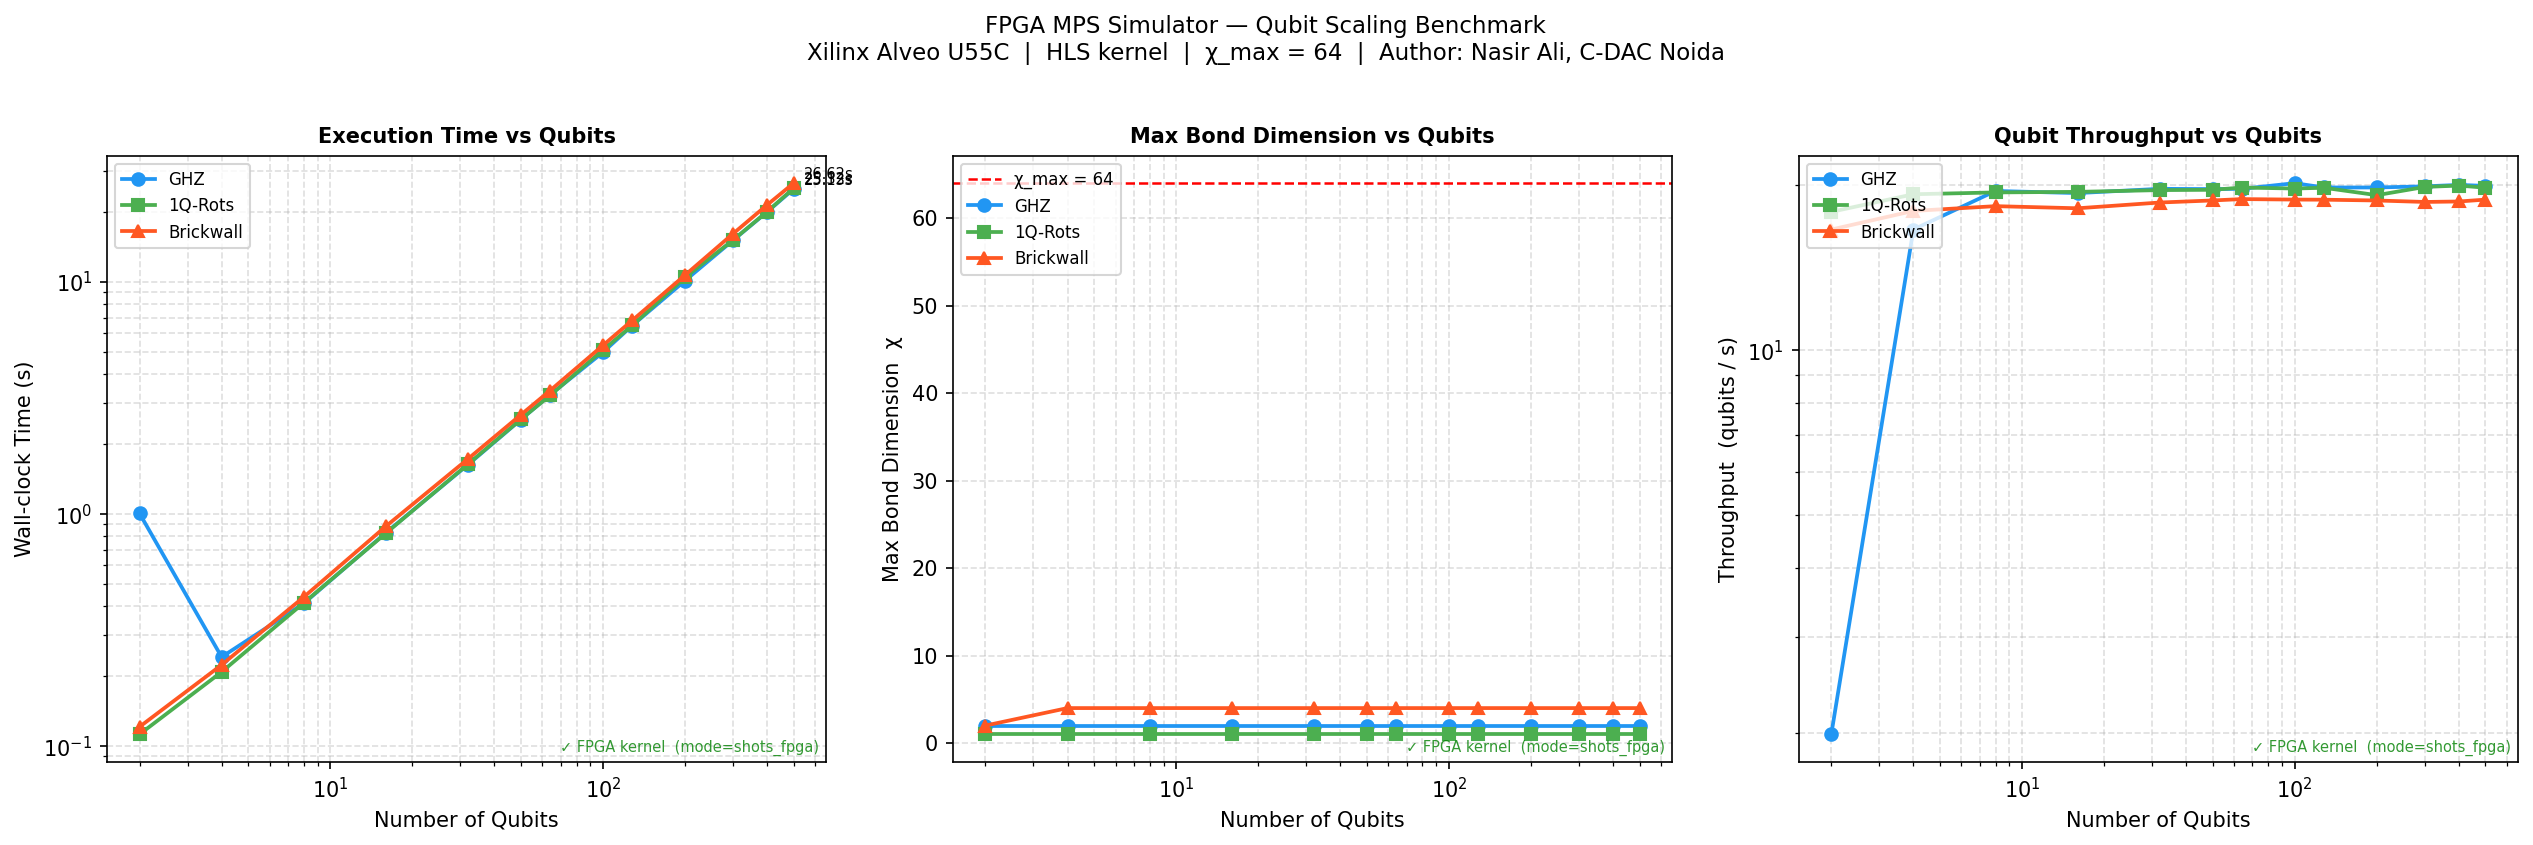
\includegraphics[width=0.8\linewidth]{figs/scaling_results.png}
  \caption{MPS simulation time vs.\ qubit count for three circuit families
           at $\chi_{\max}=64$.}
  \label{fig:mps-scaling}
\end{figure}

\begin{figure}[t]
  \centering
  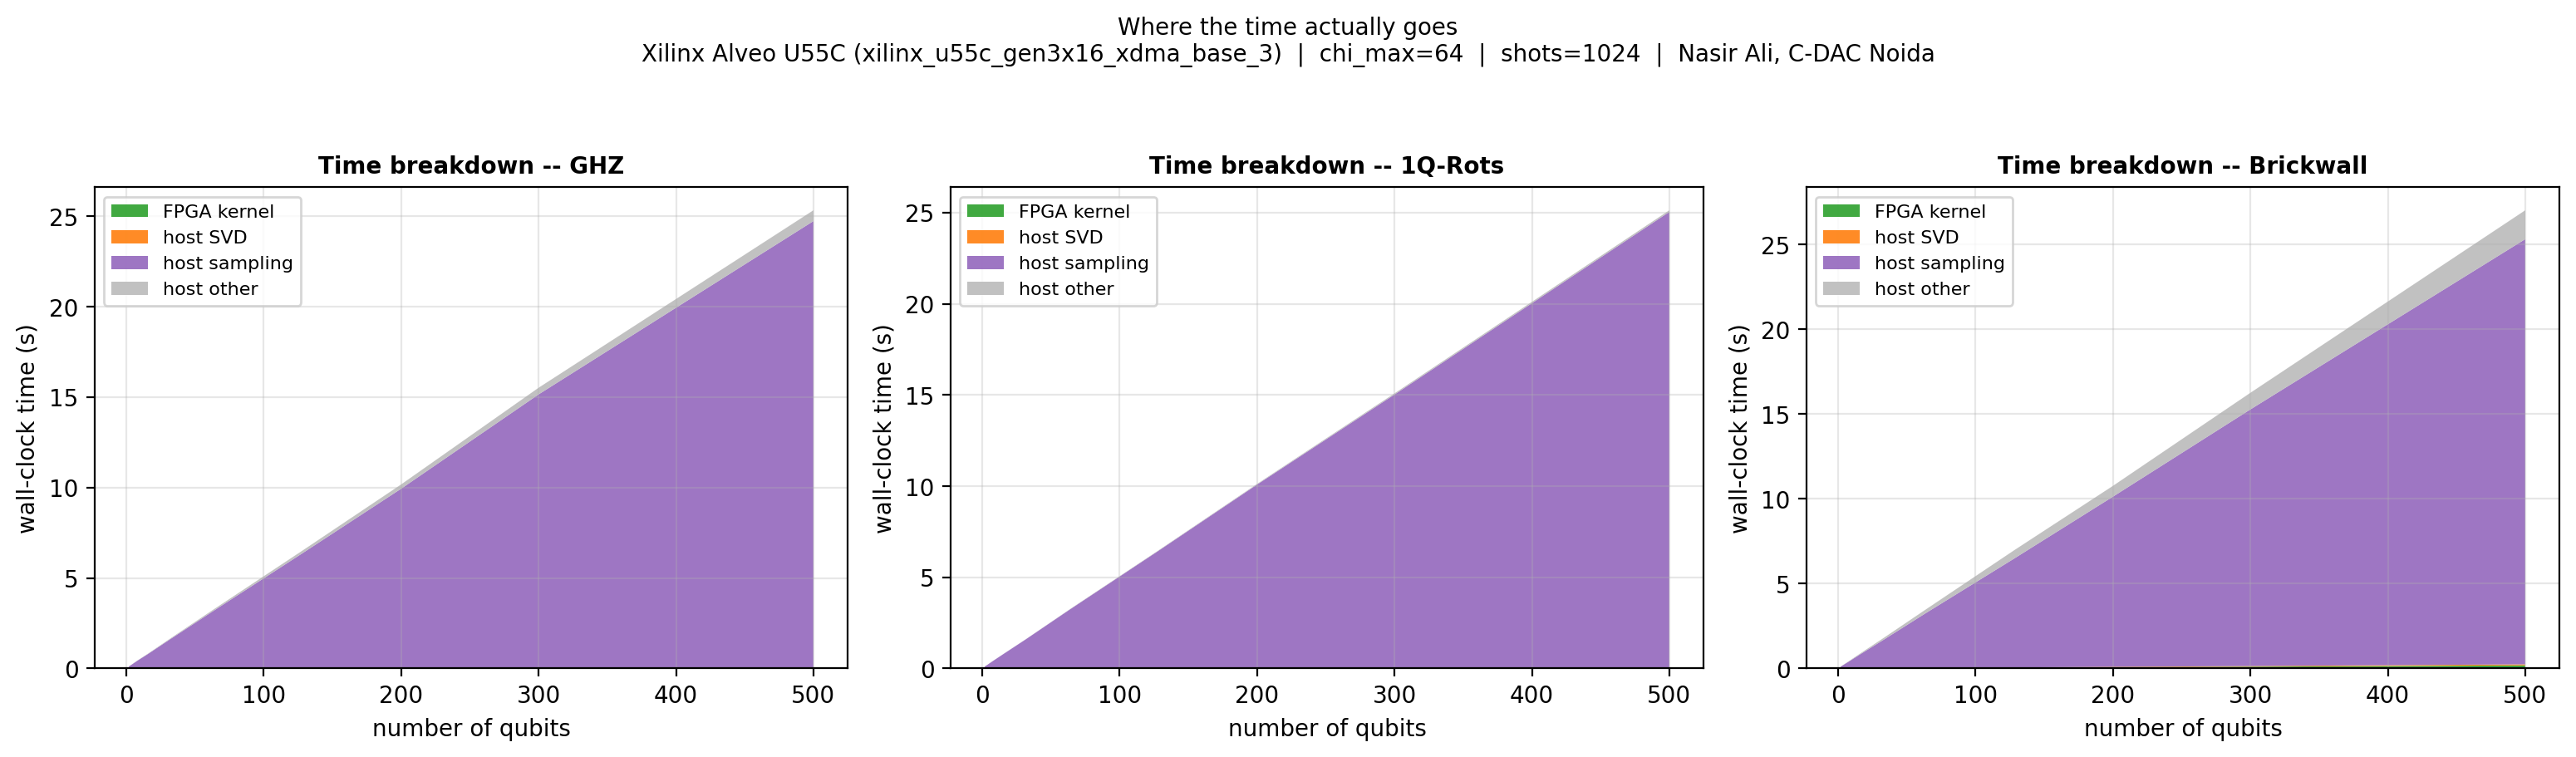
\includegraphics[width=0.8\linewidth]{figs/fig_1_time_attribution.png}
  \caption{Time attribution breakdown for MPS simulation.}
  \label{fig:time-attr}
\end{figure}

\subsection{Combined Exact-vs-MPS Fidelity}

\begin{figure}[t]
  \centering
  % \includegraphics[width=0.8\linewidth]{figs/exact_vs_mps.png}
  \caption{\TODO{Combined exact SV vs.\ MPS fidelity plot. Generate after
           Phase A and B gates are passed.}}
  \label{fig:exact-vs-mps}
\end{figure}

\subsection{Shots-Parallel Throughput}

\begin{table}[t]
\caption{Shots-parallel throughput scaling (MPS, $n=20$, $\chi_{\max}=32$,
$1024$ shots).
\TODO{Fill from results/mps\_scaling.csv}}
\label{tab:shots-parallel}
\centering
\begin{tabular}{rrrr}
\toprule
Cards & Shots/card & Wall time (s) & Speedup \\
\midrule
1 & 1024 & \TODO{} & 1.0$\times$ \\
4 & 256  & \TODO{} & \TODO{}$\times$ \\
\bottomrule
\end{tabular}
\end{table}


%%%% ============================================================
\section{Discussion}
\label{sec:discussion}
%%%% ============================================================

\textbf{Diagonal-gate insight generalises.}
The local-diagonal observation extends beyond \qft{}: any variational quantum
eigensolver (VQE) layer with parametric $R_Z$ and $C_P$ gates on partition qubits
can be executed with zero cross-card communication.
This motivates a gate-classification pre-pass for any distributed statevector engine.

\textbf{Memory wall at 28 qubits.}
At $n=28$ each of the four cards requires \SI{1.07}{\giga\byte} HBM, within the
\SI{8}{\giga\byte} budget but leaving little headroom for multi-circuit batching.
Extending to $n=32$ would require $K=16$ cards or 64-card distribution.

\textbf{AXI routing risk.}
The SV kernel's 17 AXI masters present routing congestion risk on Alveo U55C.
The MPS kernel's 9-master design serves as a validated lower-risk baseline.
Production deployments should evaluate an 8-bank SV variant as a fallback.

\textbf{MPS entanglement ceiling.}
For the brickwall circuit family, the \mps{} approximation error grows past
$n=\TODO{}$ qubits at $\chi_{\max}=64$.
Increasing $\chi_{\max}$ to 128 would require \TODO{XX} additional HBM capacity
per card and re-synthesis of the FPGA kernel.


%%%% ============================================================
\section{Limitations}
\label{sec:limitations}
%%%% ============================================================

\begin{itemize}
  \item The SV engine requires FPGA-mandatory mode; no CPU fallback.
  \item Gate parameter precision is float32 (promoted to double in-kernel);
        circuits with extremely precise angles may require a 64-bit encoding.
  \item MPS is approximate for high-entanglement circuits beyond $\chi_{\max}=64$.
  \item Routing congestion at 17 AXI masters for the SV kernel is a
        hardware risk on Alveo U55C.
\end{itemize}


%%%% ============================================================
\section{Conclusion}
\label{sec:conclusion}
%%%% ============================================================

We presented a dual-engine FPGA quantum simulator combining a distributed exact
statevector engine and an \mps{} engine on four Xilinx Alveo U55C accelerators.
The central technical contribution is the \emph{diagonal-gate local-path} insight:
all diagonal gates in a quantum circuit, including every controlled-phase gate in
the \qft{}, can be applied locally on each card without cross-card communication.
This reduces \qft{} exchange overhead from $O(n^2)$ gates to $O(1)$, enabling
28-qubit \qft{} with fidelity $\geq 1-10^{-9}$ at $n\leq 22$.
The \mps{} engine extends the simulator's reach to $500+$ qubits per card for
low-entanglement circuits with $\approx 4\times$ shots-parallel throughput.
Together, the two engines cover complementary corners of the simulation landscape
that no single prior FPGA implementation has addressed simultaneously.

\section*{Declarations}

\subsection*{Funding}
This work was supported by C-DAC, Noida under internal research funds.

\subsection*{Competing Interests}
The authors declare no competing interests.

\subsection*{Availability of Code}
Source code will be made available upon publication.

%%%% ============================================================
\bibliography{references}
%%%% ============================================================

\end{document}
